\section{Аналитическая часть}

\subsection{Составляющие компилятора}
Компилятор состоит из трёх частей.
\begin{enumerate}
	\item \textit{Frontend} преобразует текст программы на исходном языке во внутреннее представление, состоит из четырёх частей: препроцессор, лексический и синтаксический анализаторы, генератор внутреннего представления.  
	
	\item \textit{Middle-end} занимается машинно-независимой оптимизацией полученного внутреннего представления.
	
	\item \textit{Backend} выполняет преобразование внутреннего представления в программу на языке целевой платформы (ассемблер или машинный код).
\end{enumerate}

На рисунке \ref{fig:phases} изображены основные фазы работы компилятора.

\begin{figure}[h]
	\begin{center}
		{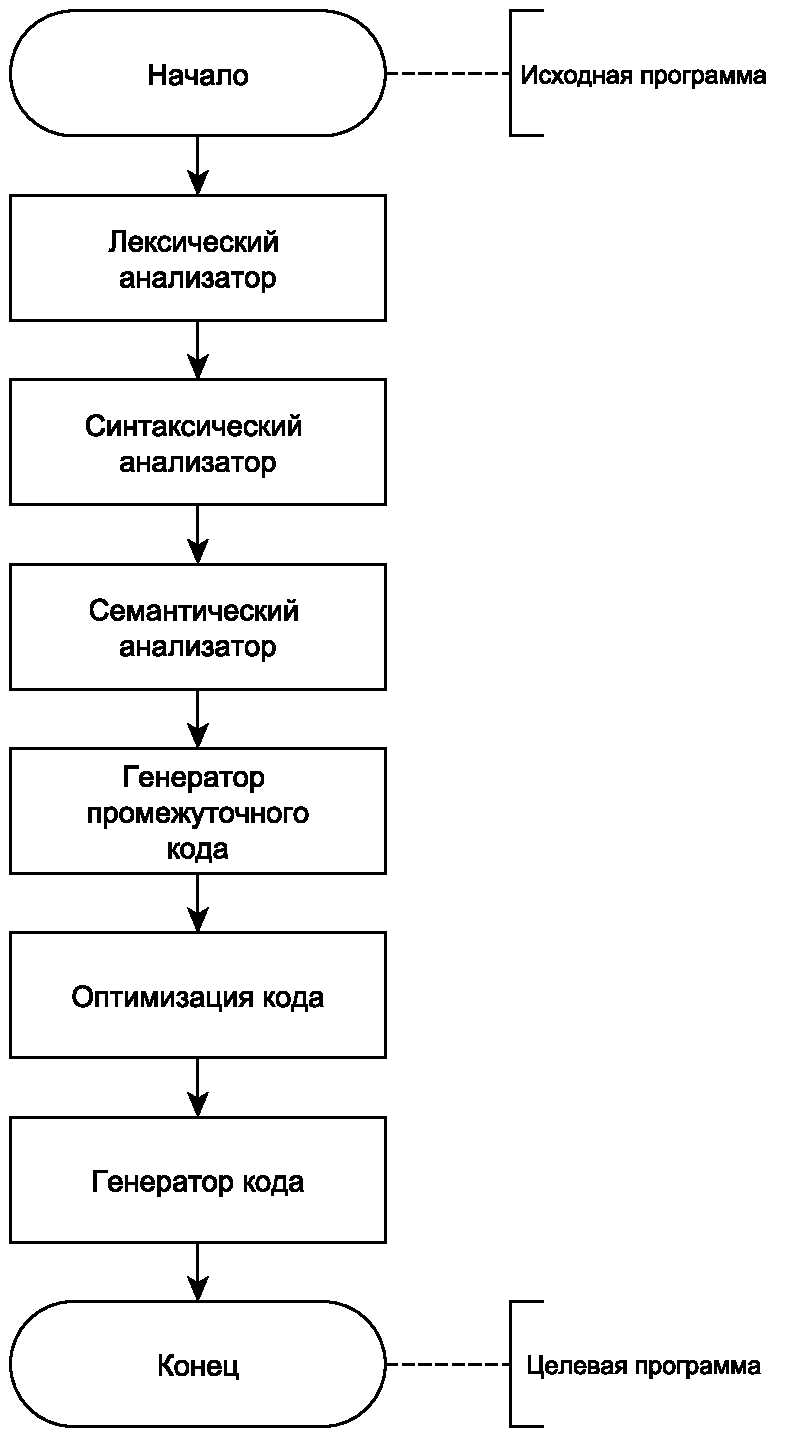
\includegraphics[scale = 0.53, page=1]{img/phases.pdf}}
		\caption{Фазы компилятора.}
		\label{fig:phases}
	\end{center}
\end{figure}

\subsubsection{Лексический анализатор}
Цель -- превратить поток символов в токены (этот процесс называется <<токенизацией>>). Выполняется группировка определённых терминальных символов в лексемы. Задаются конкретные правила в виде регулярных выражений, детерминированных конечных автоматов, грамматик. 

Лексический анализ может представляться как один из этапов синтаксического анализа. 

Обнаружение лексических ошибок, таких как недопустимые символы, ошибки идентификаторов или числовых констант, также является частью этого процесса. Кроме того, на этом этапе происходит удаление комментариев и обработка директив условной компиляции. \\

\subsubsection{Синтаксический анализатор}
Иерархический анализ называется разбором (<<parsing>>) или синтаксическим анализом, который включает группировку токенов исходной программы в грамматические фразы, используемые компилятором. Обычно они представляются в виде дерева. 

Обычно это представление выражается в виде абстрактного синтаксического дерева, где каждый внутренний узел является оператором, а дочерние -- его аргументами. Среди них можно выделить несколько групп связанных объектов:
\begin{itemize}
	\item элементы арифметических выражений: каждый узел представляет собой операцию и содержит её аргументы;
	
	\item элементы системы типов: базовые типы (числовые, строковые, структуры и т.п.), указатели, массивы и функции;
	 
	\item выражения пяти типов: арифметические, блочные и управляющие выражения, условные конструкции, циклы.
\end{itemize}

Разбор начинается со стартового нетерминала. 

Условные конструкции описывают конструкцию <<if>>, включающую в себя арифметическое выражение условия, выражение, выполняемое в случае его истинности, и альтернативное опциональное выражение.

Конструкции циклов (включают в себя <<while>>, <<do while>>, <<for>>) описывают арифметическое выражение условия и выражение, исполняемое в цикле.

Управляющие выражения -- <<break>>, <<continue>>, <<return>> и т.д. 

Блочные выражения -- последовательность других выражений, преимущественно используются в качестве тел функций и условных выражений и циклов.

Полученная грамматическая структура используется в последующих этапах компиляции для анализа исходной программы и генерации кода для целевой платформы. 

Синтаксический анализ выявляет синтаксические ошибки, относящиеся к нарушению структуры программы. \\

\subsubsection{Семантический анализатор}
В процессе семантического анализа проверяется наличие семантических ошибок в исходной программе и накапливается информация о типах для следующей стадии -- генерации кода. Используются иерархические структуры, полученные во время синтаксического анализа для идентификации операторов и операндов выражений и инструкций. 

Как правило, семантический анализатор разделяется на ряд более мелких, каждый из которых предназначен для конкретной конструкции. Соответствующий семантический анализатор вызывается синтаксическим анализатором как только он распознает синтаксическую единицу, требующую обработки.

Семантические анализаторы взаимодействуют между собой посредством информации, хранящейся в структурах данных, например, в центральной таблице символов. \\

\subsubsection{Генерация кода}
Последний этап -- генерация кода. Начинается тогда, когда во все системные таблицы занесена необходимая информация. В этом случае, компилятор переходит к построению соответствующей программы в машинном коде. Код генерируется при обходе дерева разбора, построенного на предыдущих этапах. 

Для получения машинного кода требуется два отдельных прохода:
\begin{itemize}
	\item генерация промежуточного кода;
	
	\item генерация собственно машинного кода.
\end{itemize}

Для каждого узла дерева генерируется соответствующий операции узла код на целевой платформы. В процессе анализа кода программы данные связываются с именами переменных. При выполнении генерации кода предполагается, что вход генератора не содержит ошибок. Результат -- код, пригодный для исполнения на целевой платформе. \\

\subsection{Методы реализации лексического и синтаксического анализаторов}
Существует два подхода для реализации лексического и синтаксического анализаторов:
\begin{itemize}
	\item с использованием стандартных алгоритмов анализа;
	
	\item с привлечением готовых инструментов генерации. \\
\end{itemize}

\subsubsection{Генераторы лексического анализатора}
Существует множество генераторов, наиболее популярные из них -- Lex, Flex, ANTLR4 и другие. 

\textbf{Lex} -- стандартный инструмент для получения лексических анализаторов в операционных системах Unix, обычно используется совместно с генератором синтаксических анализаторов Yacc. В результате обработки входного потока получается исходный файл на языке Си. Lex-файл разделяется на три блока (блок определений, правил и кода на Си), разделённые строками, содержащими по два символа процента. \cite{bib:lex}

В блоке определений задаются макросы и заголовочные файлы. Блок правил описывает шаблоны, представляющие собой регулярные выражения, и ассоциирует их с вызовами. Блок кода  содержит операторы и функции на Си, которые копируются в генерируемый файл.

\textbf{Flex} (Fast Lexical Analyzer) заменяет Lex в системах на базе пакетов GNU и имеет аналогичную функциональность. \cite{bib:flex}

\textbf{ANTLR} (ANother Tool for Language Recognition) -- генератор лексических и синтаксических анализаторов, позволяет создавать анализаторы на таких языках, как: Java, C\#, Python 2, Python 3, JavaScript, Go, C++, Swift, PHP. \cite{bib:antlr4}

ANTLR генерирует классы нисходящего рекурсивного синтаксического анализатора, на основе правил, заданных в виде РБНФ грамматики. Он также позволяет строить и обходить деревья синтаксического анализа с использованием паттернов посетитель или слушатель. Благодаря своей эффективности и
простоте использования, ANTLR является одним из наиболее предпочтительных генераторов анализаторов при создании кода синтаксического анализатора. В текущей работе было решено использовать этот инструмент. \\

\subsubsection{Генераторы синтаксического анализатора}
Для создания синтаксических анализаторов используются такие инструменты, как Yacc/Bison, Coco/R и описанный ранее ANTLR.

\textbf{Yacc} -- стандартный генератор синтаксических парсеров в Unix системах, \textbf{Bison} -- аналогичный ему генератор для GNU систем. \cite{bib:bison}

\textbf{Coco/R} -- генератор лексических и синтаксических анализаторов. Лексические анализаторы работают по принципу конечных автоматов, а синтаксические используют рекурсивный спуск. Поддерживаются такие языки программирования, как C++, C\#, Java и другие. \\

\subsection{LLVM}
LLVM (Low Level Virtual Machine) -- проект программной инфраструктуры для создания компиляторов и сопутствующих им утилит. В его основе лежит платформонезависимая система кодирования машинных инструкций -- байткод LLVM IR (Intermediate Representation). LLVM может создавать байткод для множества платформ, включая ARM, x86, x86-64, GPU от AMD и Nvidia и другие. В проекте есть генераторы кода для множества языков, а для компиляции LLVM IR в код платформы используется clang. В состав LLVM  входит также интерпретатор LLVM IR, способный исполнять код без компиляции в код платформы. \cite{bib:llvm}

Некоторые проекты имеют собственные LLVM-компиляторы, например, LLVM-версия GCC.

LLVM поддерживает целые числа произвольной разрядности, числа с плавающей точкой, массивы, структуры и функции. Большинство инструкций в LLVM принимает два аргумента (операнда) и возвращает одно значение (трёхадресный код).

Значения в LLVM определяются текстовым идентификатором. Локальные значения обозначаются префиксом \%, а глобальные – @. Тип операндов всегда указывается явно и однозначно определяет тип результата. Операнды арифметических инструкций должны иметь одинаковый тип, но сами инструкции «перегружены» для любых числовых типов и векторов.

LLVM поддерживает полный набор арифметических операций, побитовых логических операций и операций сдвига. LLVM IR строго типизирован, поэтому существуют
операции приведения типов, которые явно кодируются специальными инструкциями. Кроме того, существуют инструкции преобразования между целыми числами и
указателями, а также универсальная инструкция для приведения типов bitcast.

Помимо значений ­регистров в LLVM есть работа с памятью. Значения в памяти адресуются типизированными указателями. Обратиться к ней можно с помощью двух инструкций: load и store. Инструкция alloca выделяет память на стеке. Она автоматически освобождается при выходе из функции при помощи инструкций ret или unwind.

Для вычисления адресов элементов массивов и структур с правильной типизацией используется инструкция getelementptr. Она только вычисляет
адрес без обращения к памяти, принимает произвольное количество индексов и может разыменовывать структуры любой вложенности. \\

\subsection*{Выводы}
В данном разделе приведён обзор основных фаз компиляции, описана каждая из них. Также был выбран генератор лексического и синтаксического анализаторов -- ANTLR. 

\pagebreak